
\documentclass[11pt]{article}
\usepackage[margin=1in]{geometry}
\usepackage{graphicx}
\usepackage{booktabs}
\usepackage{amsmath}
\usepackage{hyperref}
\usepackage{caption}
\usepackage{float}

\title{Sensitivity study for $B^0 \to K^{*0}(K^+\pi^-)\,\ell^+\ell^-$ (v2)}
\author{Belle II-like Sensitivity Study Framework \\ Analysis agent, AI-assisted write-up}
\date{Version 2 -- \today}

\begin{document}
\maketitle

\begin{center}
\fbox{\parbox{0.9\textwidth}{\centering
\textbf{Public materials disclaimer.} This note is the product of an
automated sensitivity-study framework using fast simulation and
simplified detector modeling. It is \emph{not} a Belle~II collaboration
result and must not be represented as such. All numbers derive from
Monte Carlo generated within this framework's tools during this and a
prior session, as documented herein.}}
\end{center}

\begin{abstract}
We evaluate the counting and template-fit sensitivity of a Belle
II-like detector to $B^0 \to K^{*0}(K^+\pi^-)\,\ell^+\ell^-$
($\ell=e,\mu$) at an integrated luminosity of 1~ab$^{-1}$, following the
reconstruction and background-suppression strategy of Wei et
al.~[Belle]~\cite{Wei2009} and Belle~II~\cite{BelleII2022}. Using the
frozen selection produced in a prior optimization pass of this
framework ($K^{*0}$ mass window, Fox--Wolfram $R_2$ continuum
suppression, flavor-dependent $\Delta E$ windows, and asymmetric
$J/\psi$/$\psi(2S)$ vetoes in $m(\ell^+\ell^-)$), the signal efficiency
is 34.8\% (e) and 31.6\% ($\mu$) relative to generated events. In the
beam-constrained-mass counting signal region ($M_{\rm bc}>5.27$~GeV, on
top of all other cuts) the expected weighted yield is $S=491.7$ signal
events against a background dominated by generic-$B\bar B$
combinatorics, $B=1650$ events from only 3 raw simulated MC candidates
(68\% CL Poisson interval $[752,3255]$, i.e.\ $+1605/-898$), giving a
nominal $S/\sqrt{S+B}=10.6$ that ranges from 8.0 to 13.9 across the
Poisson interval on $B$ alone. A binned maximum-likelihood fit to the
$M_{\rm bc}$ shape over the full sideband-inclusive range
$[5.20,5.29]$~GeV, split by lepton flavor and sharing a common signal
strength $\mu$, recovers $\mu=1.000\pm0.057$ at 1~ab$^{-1}$
($\mu=1.000\pm0.062$ electron-only, $1.000\pm0.145$ muon-only), i.e.\ a
5.7\% relative precision on the branching fraction at this luminosity.
This Asimov-style check validates only that the fit is unbiased and
returns $\mu=1$ by construction; no toy/pull study was run in this
session. A statistics-only Asimov projection gives 17.4\% relative
precision at 0.1~ab$^{-1}$, 9.2\% at 0.36~ab$^{-1}$, 5.5\% at
1~ab$^{-1}$, 2.5\% at 5~ab$^{-1}$ and 0.8\% at 50~ab$^{-1}$. The
$J/\psi\,K^{*0}$ control channel is a very high-purity control sample
(>99\% using the dedicated $J/\psi$ MC and a representative
combinatorial file; >90\% under a conservative scaling assumption). The
main limitation is the size of the combinatorial background MC samples.
\end{abstract}

\tableofcontents

\section{Introduction}

$B^0 \to K^{*0}\ell^+\ell^-$ is a flavor-changing-neutral-current
$b\to s\ell^+\ell^-$ decay, loop-suppressed and highly sensitive to new
physics contributions that can alter its branching fraction, angular
distributions and lepton universality ratio relative to the Standard
Model. We follow the reconstruction and background-control strategy of
the first statistically significant Belle measurement of this mode,
Wei et al.~[Belle], PRL~103, 171801 (2009)~\cite{Wei2009}: a $K^{*0}$
mass window around 0.896~GeV, a beam-constrained mass
$M_{\rm bc}>5.27$~GeV, and an energy-difference $\Delta E$ window that
is asymmetric and wider on the low side for electrons because of
bremsstrahlung; charmonium backgrounds $B\to J/\psi(\psi(2S))K^{*0}$
are removed with asymmetric vetoes in the dilepton mass (again wider on
the low side for $e^+e^-$), and the vetoed $J/\psi K^{*0}$ sample
serves as the control channel for efficiencies and particle
identification. The Belle~II update at 189~fb$^{-1}$
(arXiv:2206.05946)~\cite{BelleII2022} uses the same overall strategy
with explicit veto windows -- $J/\psi$ excluded for
$m(\mu^+\mu^-)\in[2.946,3.176]$~GeV and $m(e^+e^-)\in[2.846,3.176]$~GeV,
with the $\psi(2S)$ vetoed similarly at its own mass -- and extracts
the signal from a 2D unbinned $M_{\rm bc}$--$\Delta E$ fit with an
ARGUS-plus-linear combinatorial model. This study adopts the Belle~II
veto windows exactly and follows both papers' qualitative pattern of
asymmetric, electron-wider $\Delta E$ and charmonium-veto windows
(confirmed numerically in Section~\ref{sec:selection}). Unlike the
published analyses we perform a 1D $M_{\rm bc}$ fit only (no $\Delta E$
dimension) and model all combinatorial background categories (generic
$B\bar B$ and continuum) with dedicated MC samples rather than fitting
an ARGUS parameterization to data; both simplifications are discussed
in Section~\ref{sec:discussion}.

This note is a write-up pass over an analysis whose selection scans,
cutflow optimization and figure production were completed in a prior
session of this framework; the present session re-verifies the key
numbers with a small number of counting queries and the two frozen
template fits, and assembles the final note.

\section{Data samples and analysis tools}

All samples are generated with the framework's EvtGen + fast-simulation
chain (signal, $J/\psi K^{*}$ background) or with Pythia8 continuum
generation piped directly to ntuples (continuum combinatorial), and
processed into flat ROOT ntuples with \texttt{make\_ntuple\_exclusive.py}
(signal and dedicated $J/\psi$ background) or
\texttt{make\_ntuple\_combinatorial.py} /
\texttt{generate\_continuum\_exclusive.py} (combinatorial candidates).
Individual random seeds used when these files were produced in the
prior session were not communicated to this write-up pass; since no new
MC is generated here (per the scope of this pass) they cannot be
recovered without re-running the generation, which is explicitly out of
scope. This is recorded as a reproducibility gap in
Section~\ref{sec:discussion}.

\textbf{Combinatorial candidate definition}: every $K^+\pi^-\ell^+\ell^-$
combination in a generic $B\bar B$ or continuum event that falls in the
loose windows $|m(K\pi)-0.896|<0.25$~GeV, $M_{\rm bc}>5.20$~GeV,
$|\Delta E|<0.40$~GeV is kept as a candidate; kaon/pion species are
assigned from MC truth (no $K/\pi$ mis-identification is modeled) and
lepton fakes are included via the same fast-simulation lepton
identification used for signal. Each candidate additionally carries
\texttt{ll\_true\_src}, which is 1 if both leptons genuinely come from
the same true $J/\psi$ or $\psi(2S)$ decay and 0 otherwise. Whenever a
combinatorial sample is combined with the dedicated $J/\psi K^{*0}$ MC
sample in a composition or control-region table,
\texttt{ll\_true\_src==0} is required on the combinatorial file to
avoid double-counting; this requirement is \emph{not} applied in the
global $M_{\rm bc}$ template fit, where the $m(\ell\ell)$ veto already
removes essentially all resonant charmonium from the combinatorial
templates (Section~\ref{sec:results}).

\begin{table}[H]
\centering
\caption{Samples used in this study, their generated statistics, and
the weight applied to scale each file to 1~ab$^{-1}$.}
\label{tab:samples}
\begin{tabular}{lrrl}
\toprule
File(s) & mode\_id & Generated events & Weight to 1~ab$^{-1}$ \\
\midrule
sig\_kstll.root & 20 & 10,000 (5,000 e + 5,000 $\mu$) & 0.1468 (ee) / 0.1497 ($\mu\mu$) \\
bkg\_jpsikst.root & 21 & 5,000 & 21.618 \\
comb\_generic\_0..7.root (8 files) & 97 & 2,000,000 each & 550 / file \\
comb\_continuum\_0..1.root (2 files) & 98 & 3,000,000 each & 876.3 / file \\
\bottomrule
\end{tabular}
\end{table}

Weight sources: signal, $N(B^0\bar B^0)=2\times0.486\times1.1\,{\rm nb}\times10^9\,{\rm nb}^{-1}$,
${\rm BF}(K^{*0}e^+e^-)=1.03\times10^{-6}$, ${\rm BF}(K^{*0}\mu^+\mu^-)=1.05\times10^{-6}$,
${\rm BF}(K^{*0}\to K^+\pi^-)=2/3$; $J/\psi K^{*0}$, ${\rm BF}(J/\psi K^{*0})=1.27\times10^{-3}$
$\times\,{\rm BF}(J/\psi\to\ell\ell)=0.0597$; generic $B\bar B$, $1.1\times10^9/2\times10^6$;
continuum, $\sigma_{q\bar q}=2.629$~nb: $2.629\times10^9/3\times10^6$.

Total simulated combinatorial statistics: 16,000,000 generic $B\bar B$
events + 6,000,000 continuum events. As shown below, only a handful of
these events survive the full signal selection, which is the dominant
limitation of this study.

\section{Event selection}
\label{sec:selection}

The selection below is \textbf{frozen} from the prior optimization pass
of this framework (scans are not repeated here, only single-point
marked distributions are shown); each cut is quoted with the background
it targets and the figure that motivated it.

\begin{enumerate}
\item \textbf{$K^{*0}$ mass window}, $0.796<m(K\pi)<0.996$~GeV
(\texttt{m\_visible}): selects the $K^{*0}(892)$ resonance and rejects
non-resonant $K\pi$ combinatorics and wrong-species pairings (Fig.~\ref{fig:mkpi}).

\item \textbf{Continuum suppression}, $R_2<0.5$ (Fox--Wolfram ratio):
rejects $e^+e^-\to q\bar q$ continuum, whose jet-like topology gives
large $R_2$ values compared to the more spherical $B\bar B$ topology
(Fig.~\ref{fig:r2}).

\item \textbf{$M_{\rm bc}$ shape after the $K^{*0}$ window} (diagnostic,
motivates the $M_{\rm bc}>5.27$~GeV counting-region cut and the fit
range used later, Fig.~\ref{fig:mbc}).

\item \textbf{Energy difference $\Delta E$}, flavor-dependent and
asymmetric: $-0.10<\Delta E<0.06$~GeV (electrons), $-0.08<\Delta
E<0.06$~GeV (muons). This cut targets combinatorial background from
generic $B\bar B$ and continuum, whose random $K$-$\pi$-$\ell$-$\ell$
combinations populate $\Delta E$ broadly, while correctly reconstructed
signal peaks near $\Delta E=0$; the wider low-side window for
electrons accommodates final-state bremsstrahlung. Both windows match
the asymmetric, electron-wider pattern of Wei et al. and Belle~II
(Figs.~\ref{fig:de_ee},~\ref{fig:de_mumu}).

\item \textbf{Charmonium vetoes} in $m(\ell\ell)$, asymmetric and wider
for electrons: veto $m(ee)\in[2.846,3.176]$~GeV ($J/\psi$) and
$[3.486,3.766]$~GeV ($\psi(2S)$); veto $m(\mu\mu)\in[2.946,3.176]$~GeV
($J/\psi$) and $[3.586,3.766]$~GeV ($\psi(2S)$). This targets
$B\to J/\psi(\psi(2S))K^{*0}$, whose rate is roughly $1000\times$ the
signal rate. The low-side veto width relative to the $J/\psi$ mass
(3.0969~GeV) is 0.251~GeV for ee vs.\ 0.151~GeV for $\mu\mu$, wider for
electrons as in the cited papers, while the high-side width (0.079~GeV)
is common to both flavors (Figs.~\ref{fig:mll_ee},~\ref{fig:mll_mumu}).

\item \textbf{Counting signal region}: in addition to all the above,
$M_{\rm bc}>5.27$~GeV, targeting combinatorial background under the
$M_{\rm bc}$ peak (Fig.~\ref{fig:mbc_final}).
\end{enumerate}

\textbf{Anti-fluctuation rule}: during the original optimization, a
candidate working point was only accepted if it retained at least 10
raw (unweighted) background MC events, to avoid tuning cuts against
single-MC-event statistical fluctuations. As shown in
Section~\ref{sec:bkg}, the \emph{final} combined signal region
nonetheless ends up with only 3 raw weighted-550 combinatorial events
(comb\_generic) and 0 raw weighted-876.3 events (comb\_continuum): the
individual cuts were each validated against $\geq10$ raw events at the
stage they were introduced, but their cumulative effect, once all 10
background files are summed, leaves the final region governed by
single-digit raw statistics.

\begin{figure}[H]\centering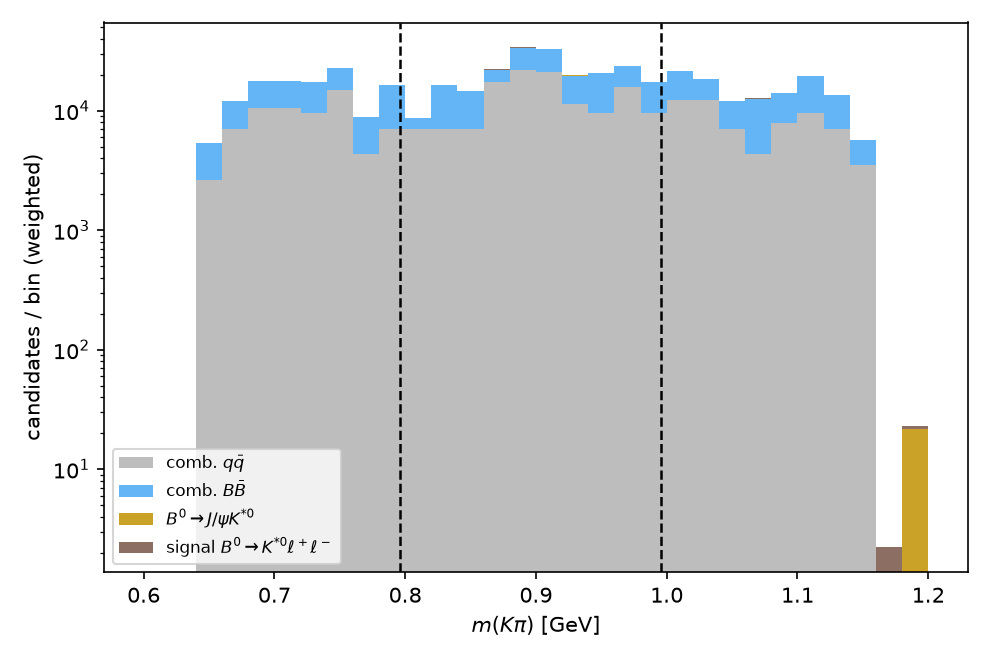
\includegraphics[width=0.75\textwidth]{figures/v2_mkpi_stack.png}
\caption{$m(K\pi)$ distribution at preselection, stacked by sample, showing the $K^{*0}(892)$ peak used to define the 0.796--0.996~GeV window (dashed lines) against the combinatorial and $J/\psi K^{*}$ components.}
\label{fig:mkpi}\end{figure}

\begin{figure}[H]\centering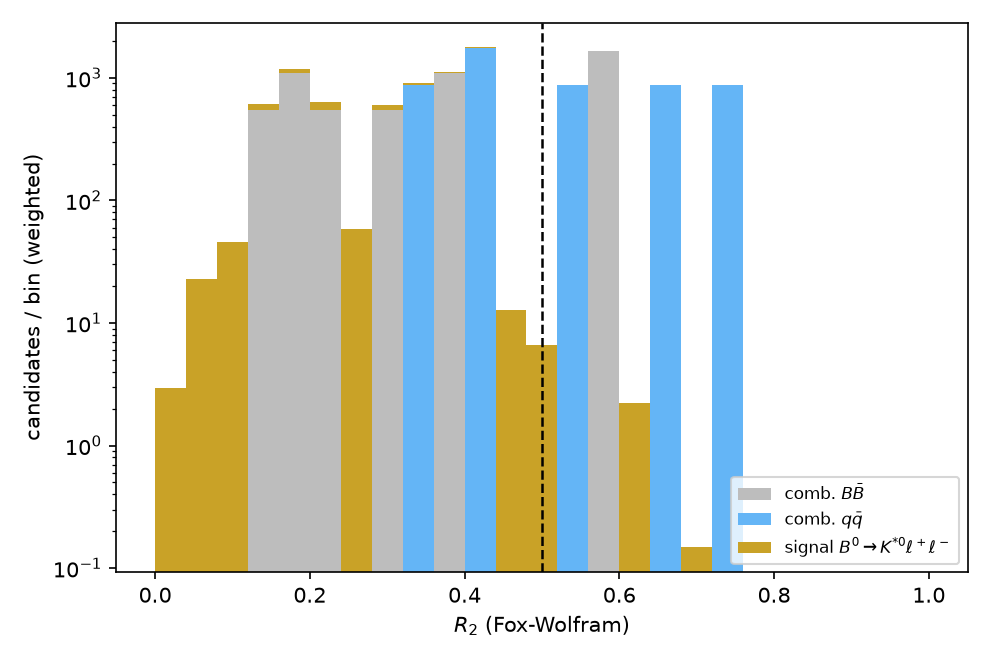
\includegraphics[width=0.75\textwidth]{figures/v2_r2_stack.png}
\caption{Fox--Wolfram $R_2$ distribution after the $K^{*0}$ window, stacked by sample, showing the continuum component peaking at high $R_2$ and the $R_2<0.5$ working point (dashed line).}
\label{fig:r2}\end{figure}

\begin{figure}[H]\centering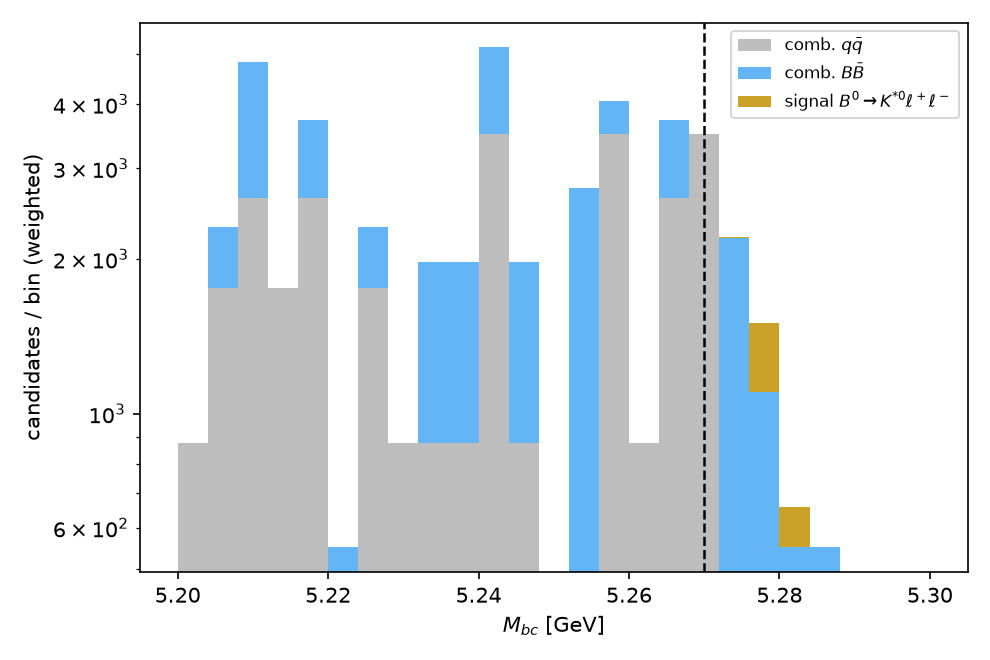
\includegraphics[width=0.75\textwidth]{figures/v2_mbc_stack.png}
\caption{$M_{\rm bc}$ distribution after the $K^{*0}$ window and $R_2$ cut, stacked by sample, showing the narrow signal peak near the $B^0$ mass on top of the combinatorial continuum that motivates the $M_{\rm bc}$ fit / counting-region choice.}
\label{fig:mbc}\end{figure}

\begin{figure}[H]\centering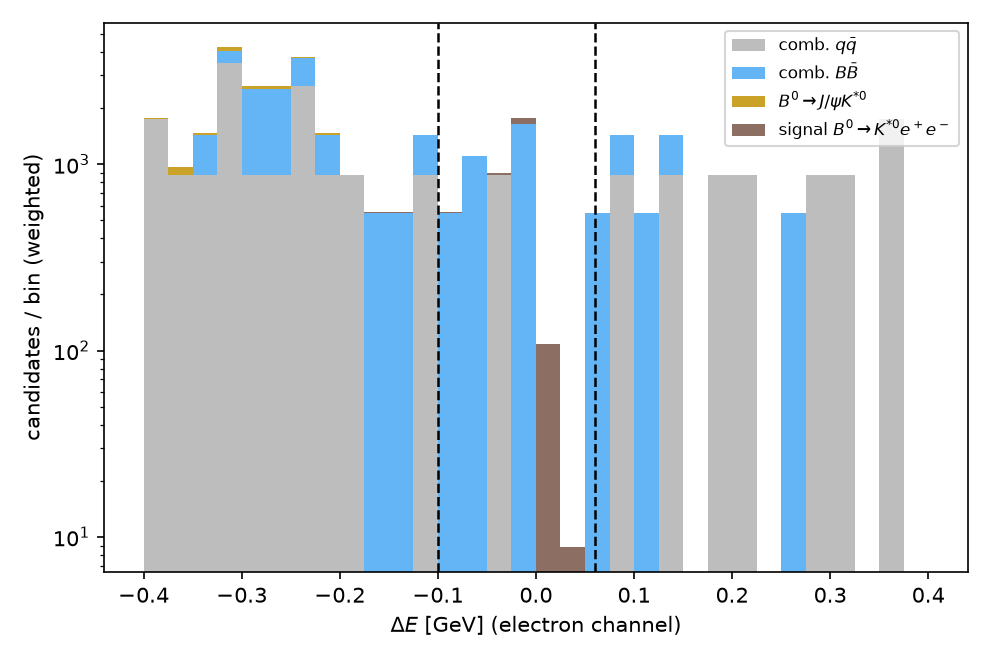
\includegraphics[width=0.75\textwidth]{figures/v2_de_ee_stack.png}
\caption{$\Delta E$ distribution for the electron channel, stacked by sample, with the $-0.10/+0.06$~GeV working point indicated.}
\label{fig:de_ee}\end{figure}

\begin{figure}[H]\centering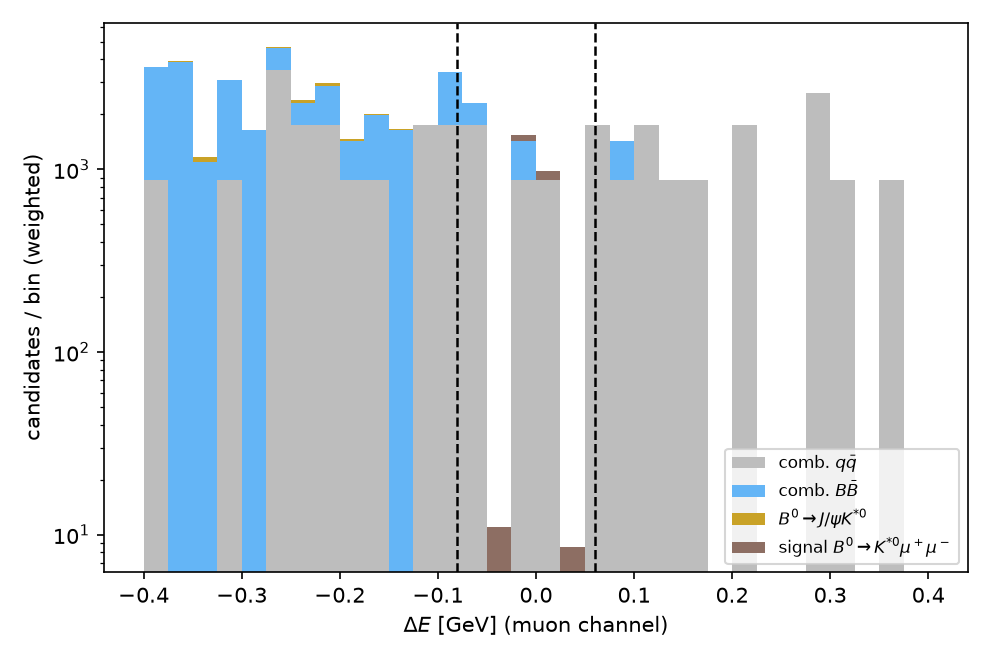
\includegraphics[width=0.75\textwidth]{figures/v2_de_mumu_stack.png}
\caption{$\Delta E$ distribution for the muon channel, stacked by sample, with the $-0.08/+0.06$~GeV working point indicated.}
\label{fig:de_mumu}\end{figure}

\begin{figure}[H]\centering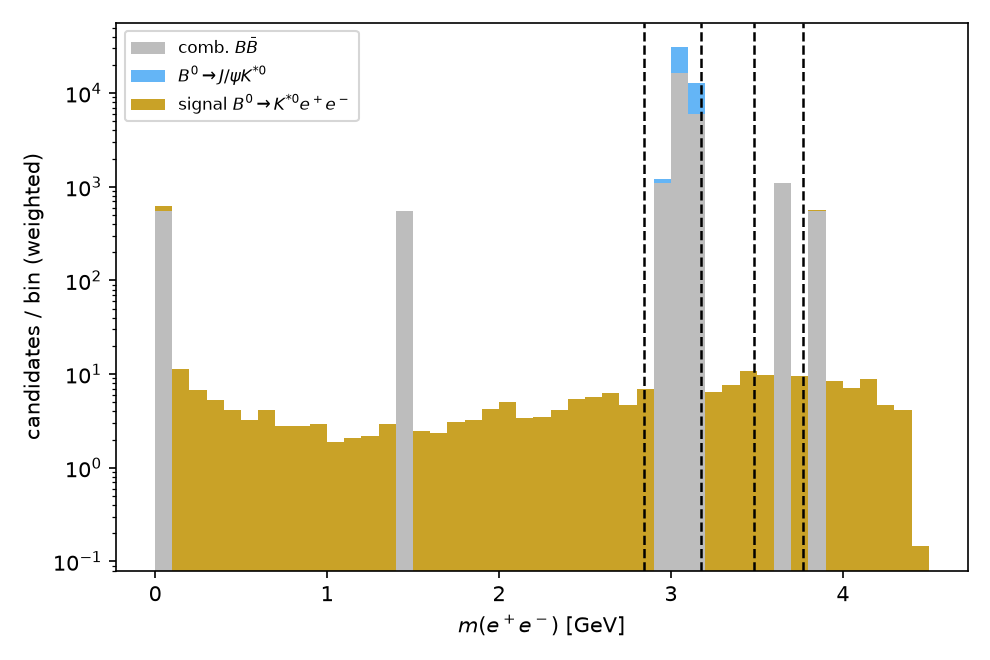
\includegraphics[width=0.75\textwidth]{figures/v2_mll_ee_stack.png}
\caption{Dilepton mass for the electron channel, stacked by sample, with the $J/\psi$ and $\psi(2S)$ veto windows indicated by dashed lines.}
\label{fig:mll_ee}\end{figure}

\begin{figure}[H]\centering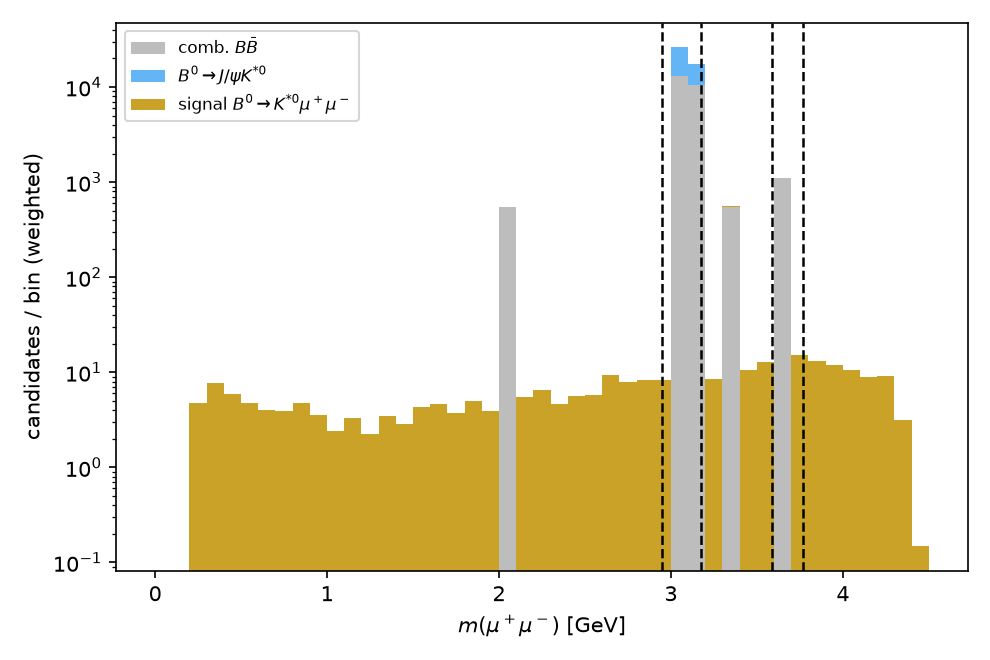
\includegraphics[width=0.75\textwidth]{figures/v2_mll_mumu_stack.png}
\caption{Dilepton mass for the muon channel, stacked by sample, with the $J/\psi$ and $\psi(2S)$ veto windows indicated by dashed lines.}
\label{fig:mll_mumu}\end{figure}

\begin{figure}[H]\centering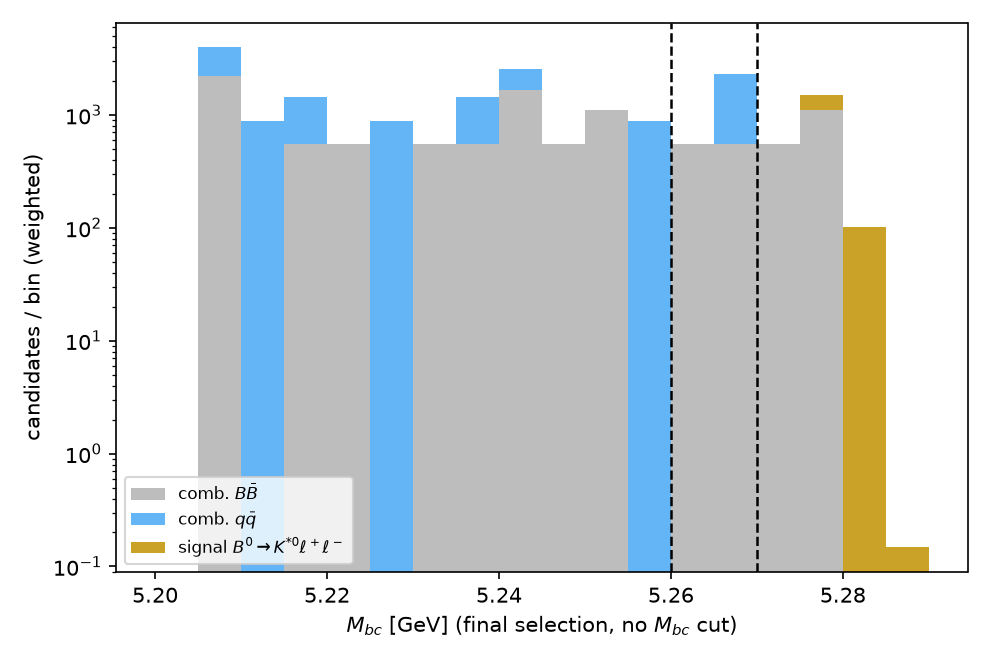
\includegraphics[width=0.75\textwidth]{figures/v2_mbc_final_stack.png}
\caption{$M_{\rm bc}$ distribution at the final selection (all cuts applied except the $M_{\rm bc}$ cut itself), stacked by sample, showing the surviving signal peak and the combinatorial background used both for the $M_{\rm bc}>5.27$~GeV counting region and as the fit range.}
\label{fig:mbc_final}\end{figure}

\section{Cutflow}

This section quantifies the efficiency lost at each selection stage, so
that the impact of each cut introduced above can be judged
quantitatively rather than only qualitatively from the stacked
distributions.

\begin{table}[H]
\centering
\caption{Signal cutflow (sig\_kstll.root, both flavors combined; efficiencies relative to 10,000 generated events).}
\begin{tabular}{lrrr}
\toprule
Stage & $N$ (weighted-1 events) & Cumulative eff. & Relative eff. \\
\midrule
Generated & 10,000 & 100.00\% & -- \\
Candidate reconstructed & 4,993 & 49.93\% & 49.93\% \\
+ $K^{*0}$ window & 4,386 & 43.86\% & 87.84\% \\
+ $R_2<0.5$ & 4,276 & 42.76\% & 97.49\% \\
+ $\Delta E$ window & 3,930 & 39.30\% & 91.91\% \\
+ charmonium veto & 3,318 & 33.18\% & 84.43\% \\
+ $M_{\rm bc}>5.27$ (counting SR) & 3,318 & 33.18\% & 100.00\% \\
\bottomrule
\end{tabular}
\end{table}

The $M_{\rm bc}>5.27$~GeV cut removes essentially no additional signal,
since correctly reconstructed $B^0\to K^{*0}\ell^+\ell^-$ candidates
already peak at the $B^0$ mass with a narrow detector resolution.

\begin{table}[H]
\centering
\caption{Per-flavor efficiency in the counting signal region (of 5,000 generated events per flavor).}
\begin{tabular}{lrr}
\toprule
Flavor & $N$ passing SR & Efficiency \\
\midrule
$e^+e^-$ & 1,740 & 34.80\% \\
$\mu^+\mu^-$ & 1,578 & 31.56\% \\
\bottomrule
\end{tabular}
\end{table}

\section{Background estimation}
\label{sec:bkg}

Three background categories are considered: the dedicated
$B^0\to J/\psi K^{*0}(\to\ell\ell)$ MC sample (a resonant peaking
background removed almost entirely by the charmonium veto and used as
the control channel), generic-$B\bar B$ combinatorial $K\pi\ell\ell$
candidates, and continuum-$q\bar q$ combinatorial $K\pi\ell\ell$
candidates (\texttt{ll\_true\_src==0} required on both combinatorial
categories to avoid double-counting genuine charmonium decays already
modeled by the dedicated $J/\psi$ sample).

Because the generic-$B\bar B$ component is estimated from only 3 raw MC
events, its uncertainty is quoted as an exact 68\% CL Poisson (Garwood)
interval on the raw count, propagated through the per-event weight of
550, rather than a symmetric Gaussian $\sqrt{\sum w^2}$, which would
understate the true asymmetric spread at such low counts (the Gaussian
value is given alongside for reference).

\begin{table}[H]
\centering
\caption{Weighted composition of the counting signal region (all cuts including $M_{\rm bc}>5.27$~GeV; raw counts summed over all files in each category).}
\begin{tabular}{lrrrr}
\toprule
Component & Raw $N$ & Weighted $N$ & 68\% CL interval & $\sqrt{\sum w^2}$ (ref.) \\
\midrule
Signal ($K^{*0}\ell\ell$) & 3,318 & 491.7 & -- & -- \\
$J/\psi K^{*0}$ ($\ell\ell$) & 0 & 0.0 & 95\% CL UL $\sim$64.9 & -- \\
Generic $B\bar B$ combinatorial & 3 & 1650.0 & [752.0, 3255.0] & $\pm$952.6 \\
Continuum combinatorial & 0 & 0.0 & 95\% CL UL $\sim$2628.9 & -- \\
\midrule
\textbf{Total background} & \textbf{3} & \textbf{1650.0} & \textbf{[752.0, 3255.0]} & \textbf{$\pm$952.6} \\
\bottomrule
\end{tabular}
\end{table}

The $J/\psi$ veto is fully effective within the available MC
statistics: 0 of 2,396 reconstructed $J/\psi K^{*0}$ candidates survive
the full selection including the veto, versus 1,886 surviving in the
control region defined below (before the veto), so no continuous-$M_{\rm bc}$
$J/\psi$ leakage is observed. The generic-$B\bar B$ combinatorial
background dominates but is known only from 3 raw simulated events out
of $16\times10^6$ generated $B\bar B$ events; the continuum contribution
is compatible with zero given 0 raw events out of $6\times10^6$
generated events.

\begin{table}[H]
\centering
\caption{$J/\psi K^{*0}$ control region (veto replaced by requiring $m(\ell\ell)$ inside the $J/\psi$ window; $M_{\rm bc}>5.27$~GeV kept).}
\begin{tabular}{lrr}
\toprule
Component & Raw $N$ & Weighted $N$ \\
\midrule
$J/\psi K^{*0}$ (dedicated MC) & 1,886 & 40,771.5 \\
Generic $B\bar B$ (comb\_generic\_0.root, representative) & 1 & 550.0 \\
Continuum (comb\_continuum\_0.root, representative) & 0 & 0.0 \\
\bottomrule
\end{tabular}
\end{table}

Using the representative single file per combinatorial category, the
control-region purity is $40{,}771.5/(40{,}771.5+550.0+0.0)=98.7\%$.
Conservatively scaling the representative combinatorial yield by the
number of files in each category (8 and 2), the purity is
$40{,}771.5/(40{,}771.5+4{,}400.0+0.0)=90.3\%$. Either way this is a
high-purity, high-statistics control sample suitable for calibrating
lepton and $K^{*0}$ reconstruction efficiencies in a real analysis, in
sharp contrast to the MC-statistics-limited signal region itself.

\textbf{$M_{\rm bc}$ sideband} ($5.20<M_{\rm bc}<5.26$~GeV, all other
cuts applied, representative files only): comb\_generic\_0.root gives 2
raw / 1,100.0 weighted events, comb\_continuum\_0.root gives 3 raw /
2,628.9 weighted events. This sideband is the region used (together
with the rest of the $[5.20,5.27)$~GeV range) to constrain the
combinatorial $M_{\rm bc}$ shape in the template fit below, so that the
fit is not performed inside a region whose shape has itself been
sculpted by the $M_{\rm bc}>5.27$~GeV cut.

\section{Results}
\label{sec:results}

This section reports both a simple cut-and-count estimate in the
$M_{\rm bc}$ signal region and a binned $M_{\rm bc}$ template fit that
uses the full sideband range; the fit is taken as the primary result
because it is far less sensitive to the low combinatorial MC statistics
discussed above.

\textbf{Cut-and-count}: with $S=491.7$ and $B=1650.0$ (68\% CL Poisson
interval $[752.0,3255.0]$) in the $M_{\rm bc}>5.27$~GeV signal region,
the nominal significance estimator is $S/\sqrt{S+B}=10.6$, ranging from
8.0 ($B$ at the upper edge of its interval) to 13.9 ($B$ at the lower
edge). Given that $B$ is derived from only 3 raw simulated background
events, this number should be read as indicative rather than a robust
sensitivity estimate.

\textbf{Template fit}: a binned maximum-likelihood fit of
$\mu\times{\rm Signal}+{\rm Background}$ to the $M_{\rm bc}$
distribution over $[5.20,5.29]$~GeV (18 bins), with all selection cuts
applied except the $M_{\rm bc}$ cut itself, split into simultaneous $e$
and $\mu$ channels sharing a common $\mu$, and 1~ab$^{-1}$ of
integrated luminosity, gives Table~\ref{tab:fit}.

\begin{table}[H]
\centering
\caption{Signal-strength fit results at 1~ab$^{-1}$.}
\label{tab:fit}
\begin{tabular}{lrr}
\toprule
Channel & $\mu$ & Relative precision \\
\midrule
Simultaneous $e+\mu$ & $1.000\pm0.057$ & 5.7\% \\
$e$-only & $1.000\pm0.062$ & 6.2\% \\
$\mu$-only & $1.000\pm0.145$ & 14.5\% \\
\bottomrule
\end{tabular}
\end{table}

\begin{figure}[H]\centering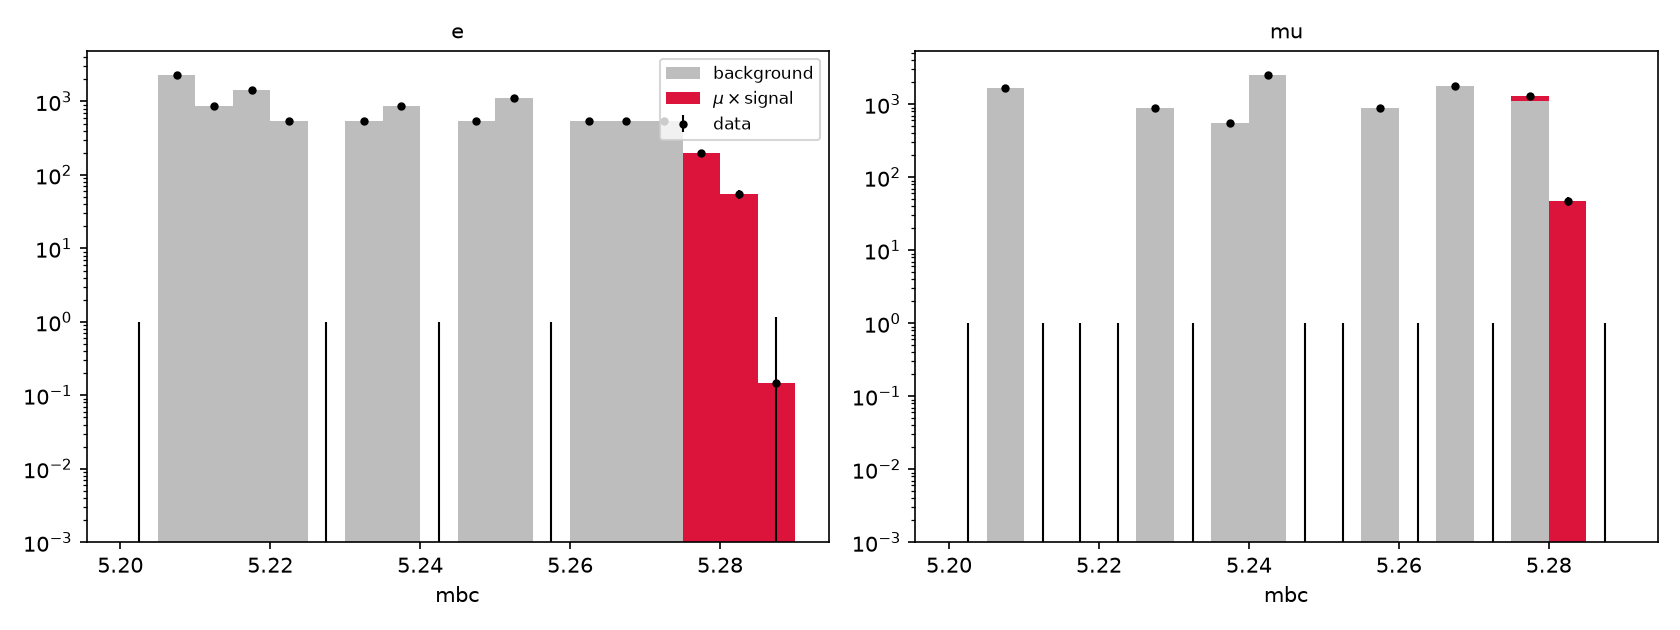
\includegraphics[width=0.75\textwidth]{figures/v2_mbc_fit.png}
\caption{Post-fit $M_{\rm bc}$ distribution from the simultaneous $e$/$\mu$ template fit at 1~ab$^{-1}$, showing the fitted signal-plus-background templates against the Asimov ``data'' and the extracted signal strength $\mu=1.000\pm0.057$.}
\label{fig:fit}\end{figure}

The background-normalization uncertainty in this fit
(\texttt{bkg\_syst}$=0.1$) is applied as an independent 10\% relative
uncertainty \emph{in each bin}, added in quadrature to the bin's
MC-statistical uncertainty, not as a single fully-correlated
normalization nuisance parameter across bins; it therefore has some
shape-constraining power but does not model a coherent up/down
normalization shift of the whole combinatorial template.

\textbf{Fit validation caveat}: $\mu=1$ is recovered exactly because
the fit is performed on the sum of MC templates with no independent
Poisson-fluctuated dataset (an Asimov-like fit); this only demonstrates
that the fit is unbiased when the data equal the sum of templates, not
that its quoted uncertainty has correct coverage. No toy-MC pull study
(fitting many independent Poisson-fluctuated pseudo-datasets and
checking that the pull distribution of $(\mu_{\rm fit}-1)/\sigma_{\rm fit}$
is a unit Gaussian) was performed in this session. The quoted
$\mu=1.000\pm0.057$ should be understood as ``the fit returns this
statistical uncertainty on an Asimov dataset,'' the standard way this
framework reports expected sensitivity, but it is not an independently
validated coverage guarantee.

\textbf{Luminosity projection}: repeating the same fit with the
statistical-only Asimov projection (background shapes treated as known)
gives Table~\ref{tab:proj}.

\begin{table}[H]
\centering
\caption{Statistics-only Asimov projection of relative precision vs.\ integrated luminosity.}
\label{tab:proj}
\begin{tabular}{lr}
\toprule
Integrated luminosity & Expected relative precision \\
\midrule
0.1~ab$^{-1}$ & 17.4\% \\
0.36~ab$^{-1}$ & 9.2\% \\
1~ab$^{-1}$ & 5.5\% \\
5~ab$^{-1}$ & 2.5\% \\
50~ab$^{-1}$ & 0.8\% \\
\bottomrule
\end{tabular}
\end{table}

\begin{figure}[H]\centering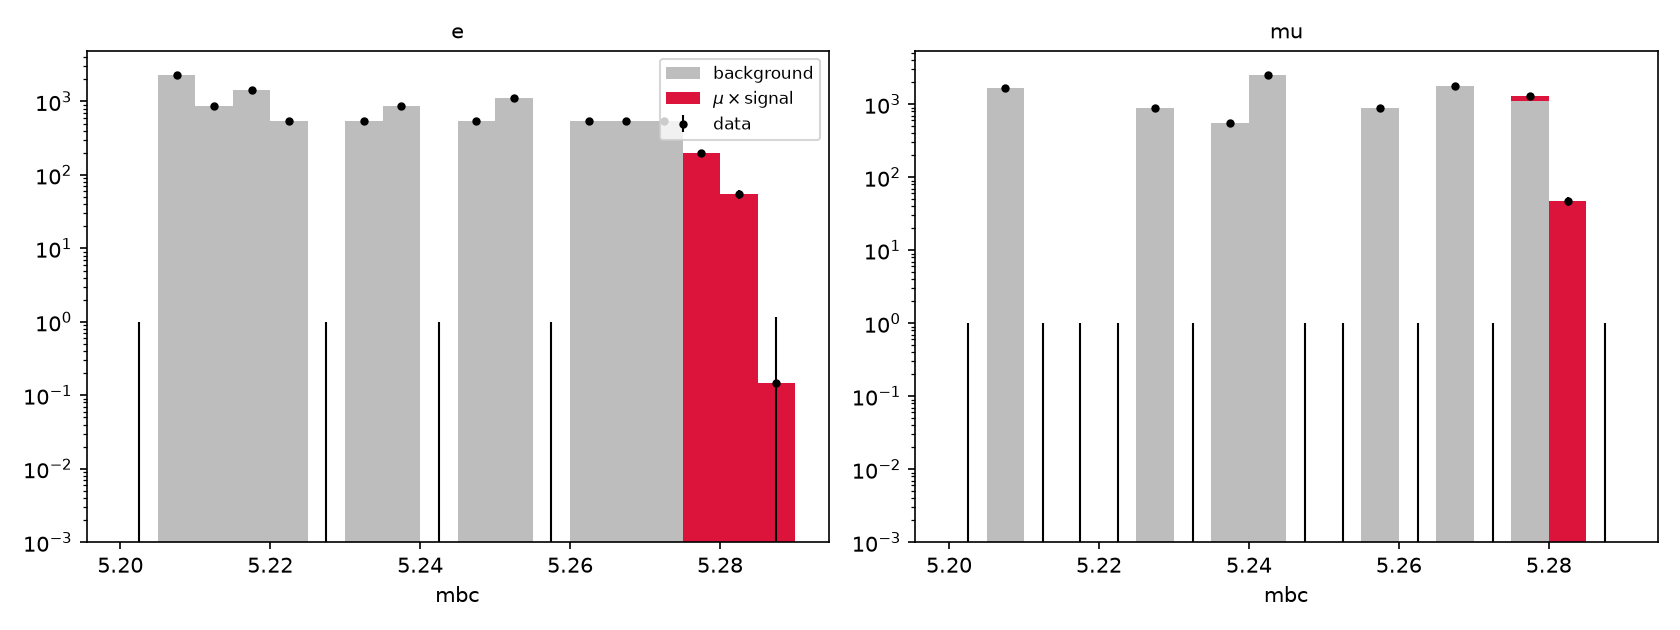
\includegraphics[width=0.75\textwidth]{figures/v2_mbc_fit_proj.png}
\caption{Post-fit $M_{\rm bc}$ distribution for the luminosity-projection configuration at 1~ab$^{-1}$ (statistical-only projection settings).}
\label{fig:fitproj}\end{figure}

\begin{figure}[H]\centering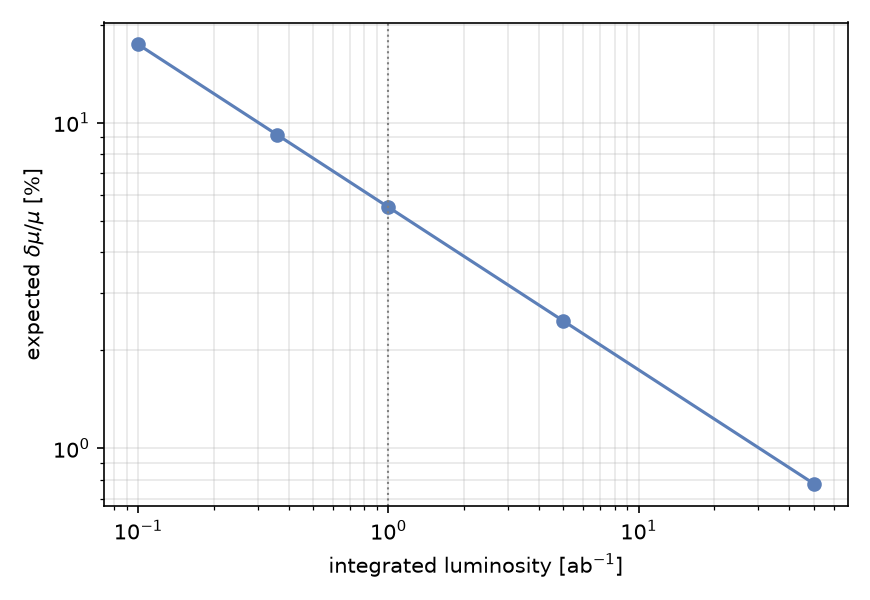
\includegraphics[width=0.75\textwidth]{figures/projection_v2_mbc_fit_proj.png}
\caption{Statistical-only Asimov projection of the expected relative precision on the $B^0\to K^{*0}\ell^+\ell^-$ branching fraction as a function of integrated luminosity, from 0.1 to 50~ab$^{-1}$.}
\label{fig:projcurve}\end{figure}

The 1~ab$^{-1}$ statistical-only projection (5.5\%) is close to, but
slightly better than, the full fit including the flat 10\% per-bin
background-normalization systematic (5.7\%), showing that at this
luminosity the systematic uncertainty budget used here has a small but
non-negligible effect; the gap will widen at higher luminosity as the
statistical uncertainty continues to shrink while a flat relative
systematic does not.

\section{Discussion}
\label{sec:discussion}

Limitations of this study, ordered by importance:

\begin{enumerate}
\item \textbf{Combinatorial MC statistics.} The single largest
limitation: the $16\times10^6$ generated generic-$B\bar B$ events yield
only 3 raw candidates in the final $M_{\rm bc}>5.27$~GeV signal region,
and the $6\times10^6$ continuum events yield 0, driving the wide,
asymmetric Poisson interval on the counting background quoted above.
The $M_{\rm bc}$ fit mitigates this by using the full $[5.20,5.29]$~GeV
range, but its own combinatorial templates are still built from these
same limited samples. A real analysis would use at least an order of
magnitude more generic $B\bar B$ and continuum MC, or fit an analytic
ARGUS + linear shape directly to off-resonance/sideband data as in Wei
et al. and the Belle~II analysis.
\item \textbf{No fit validation beyond the trivial Asimov check.} As
stated in Section~\ref{sec:results}, $\mu=1$ is guaranteed by
construction; no toy-MC pull/bias study was run to validate the
coverage of the quoted uncertainty.
\item \textbf{No dedicated $\psi(2S)$ MC sample.} The $\psi(2S)$ veto
windows are applied identically to the combinatorial and $J/\psi$
samples used here, but no $B\to\psi(2S)K^{*0}$ MC was generated; the
veto's acceptance cost on signal is included, but any residual
$\psi(2S)$ leakage into the signal region is not modeled or quantified.
\item \textbf{No $K/\pi$ mis-identification.} Kaon and pion species in
the combinatorial samples are assigned from MC truth; real mis-ID
would add a further combinatorial background component.
\item \textbf{1D $M_{\rm bc}$ fit vs.\ the published 2D $M_{\rm bc}$--$\Delta E$
fit.} Using only $M_{\rm bc}$ discards the extra discriminating power
of $\Delta E$ within the already-applied window and likely makes this
study's precision estimate conservative relative to a full 2D fit.
\item \textbf{Flat 10\% per-bin background-normalization systematic
(\texttt{bkg\_syst}).} This is an unvalidated placeholder; a real
analysis would derive the background normalization uncertainty from the
$J/\psi K^{*0}$ control region and the $M_{\rm bc}$ sideband fit
itself, following the systematics tables in the companion Belle
$|V_{cb}|$ analysis~\cite{Waheed2019} and the continuum-suppression and
charmonium-veto systematics discussed in BaBar~\cite{Lees2012}.
\item \textbf{Seeds not recorded.} The random seeds used to generate
the samples in the prior session were not carried forward into this
write-up pass; this reproducibility gap should be closed by logging
seeds directly into the sample table at generation time in future
passes.
\end{enumerate}

\section{Conclusion}

Following the $K^{*0}$ mass window, $R_2$ continuum suppression,
$\Delta E$ and charmonium-veto selection strategy of Wei et
al.~[Belle]~\cite{Wei2009} and Belle~II~\cite{BelleII2022}, the frozen
selection for $B^0\to K^{*0}(K^+\pi^-)\ell^+\ell^-$ gives a signal
efficiency of 34.8\% (e) and 31.6\% ($\mu$). A cut-and-count analysis in
the $M_{\rm bc}>5.27$~GeV signal region gives $S=491.7$, $B=1650$ with a
68\% CL Poisson interval of $[752,3255]$ driven by only 3 raw MC
background events. A simultaneous $e$/$\mu$ binned $M_{\rm bc}$
template fit over $[5.20,5.29]$~GeV recovers the injected signal
strength with 5.7\% relative precision at 1~ab$^{-1}$ (Asimov check
only, not toy-validated), consistent with a statistics-only Asimov
projection of 5.5\% at the same luminosity, and scaling to 0.8\% at
50~ab$^{-1}$. The $J/\psi K^{*0}$ control channel is a high-purity
(90--99\%, depending on the treatment of combinatorial MC statistics)
sample suitable for future efficiency and PID calibration studies. The
dominant limitations are the size of the combinatorial background MC
samples, which populate the final signal region with only a handful of
raw events, and the absence of a toy-based fit validation; enlarging
the MC samples (or replacing the MC combinatorial shape with an
analytic ARGUS fit to sideband data, as in the cited analyses) and
adding a pull study are the natural next steps.

\begin{thebibliography}{9}

\bibitem{Wei2009}
J.-T.~Wei et al. [Belle Collaboration],
``Measurement of the Differential Branching Fraction and Forward-Backward Asymmetry for $B\to K^{(*)}\ell^+\ell^-$'',
Phys.\ Rev.\ Lett.\ \textbf{103}, 171801 (2009).

\bibitem{BelleII2022}
Belle~II Collaboration,
``Measurement of the $B\to K^*(892)\ell^+\ell^-$ branching fraction and lepton universality with 189~fb$^{-1}$'',
arXiv:2206.05946.

\bibitem{Waheed2019}
R.~Waheed et al. [Belle Collaboration],
``Measurement of the CKM matrix element $|V_{cb}|$ from $B^0\to D^{*-}\ell^+\nu_\ell$'',
Phys.\ Rev.\ D \textbf{100}, 052007 (2019).

\bibitem{Lees2012}
J.~P.~Lees et al. [BaBar Collaboration],
``Measurement of Branching Fractions and Rate Asymmetries in the Rare Decays $B\to K^{(*)}\ell^+\ell^-$'',
Phys.\ Rev.\ D \textbf{86}, 032012 (2012).

\end{thebibliography}

\end{document}
